\chapter{Introduction}\label{chap:introduction}

Todays internet is no longer controlled by few standard bodies, telecommunications companies and hardware vendors. 
New Internet applications are developed by start ups at an increasing rate, and each application has the potential to disrupt the status quo, both in business and technology.
These new applications not only impact the network infrastructure, but also a large set of Stakeholders participating in todays ecosystem of applications.

Signalling Storm!


Network operator: Can manipulate network configuration, influences connection state of UE, which has an impact on power drain and thus battery life of UE.

Application Provider: Develops and deploys applications. Is usually interrested in increasing \gls{QoE} for the user. Additional considered \glspl{KPI} are cost, for example incurred due to use of compute or network resources in \gls{IaaS} or \gls{PaaS} scenarios. Design and configuration of applications has impact on traffic patterns which, result in signalling traffic in the network operators traffic and also influence the connection state of the UE.

Hardware vendor: Theoretically implements standards proposed by \gls{3GPP} in order to establish connectivity with mobile networks. However, in reality vendors are free to deviate from standard, in order increase own \glspl{KPI}. One example of such a deviation from a standard is the proprietary fast dormancy algorithm implemented by some hardware vendors. This algorithm reduces power drain be disconnecting the \gls{UE} earlier from the network. However, this has the consequence of increased signalling in the network and can result in increased page load times, i.e. decreased \gls{QoE} from the users point of view.

User uses \gls{UE} and set of applications in the network of network operator. 
%satz macht mich nicht glücklich
Usually wants to increase \gls{QoE}, i.e. by minimising power drain of \gls{UE}or increase video \gls{QoE}.

Cloud operator: Provides services to cloud users according to specified \glspl{SLA}. Wants to reduce costs to operate infrastructure, e.g. by reducing energy consumption.

NFV operator

Crowdsourcing platform operator:

CS Employer

CS Worker

%\section{Considered Stakeholders}
\section{Scientific Contribution}
This monograph studies the interactions between different stakeholders in three, partially overlapping, scenarios in order to paint a broad picture of todays interlocking network and application ecosystem.

\begin{figure}
\centering
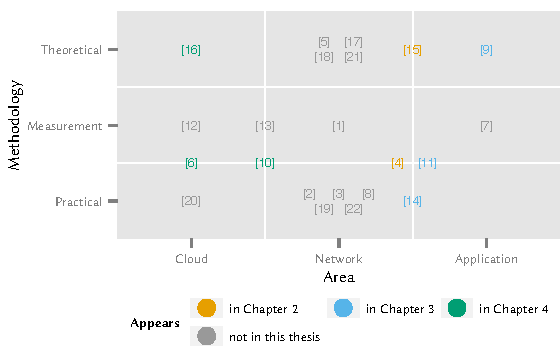
\includegraphics{figures/publications}
\caption{Contribution of this work as a classification of the research studies conducted by the author}\label{fig:introduction:publications}
\end{figure}

In \reffig{fig:introduction:publications}

The first contribution of this monograph is a study of the impact of mobile application traffic on mobile communication networks, especially considering the current network parameter selection.
To this end, we introduce an algorithm to infer power drain and generated signalling messages for a given application traffic trace and network generation.
We then extend on this algorithm and present a theoretical model to derive said metric from arbitrary \gls{IID} traffic arrival distributions.
Using these methods we study the impact of different traffic types and study the potential of network parameter optimisation as a mean to reduce signalling traffic.

As a second contribution, we provide models for two popular applications, i.e. Video Streaming and Cloud File Synchronisation, thus enabling the study of the impact of different mechanisms implemented in said applications.
For the Video Streaming application we use a simulation in order to compare \glspl{KPI} for all stakeholders in this scenario.
We show, that the Streaming mechanism allows the most flexible configuration and can provide a pareto optimal results for all pairs of metrics.
However, further study shows that in fact no pareto optimal value exists which satisfies the \glspl{KPI} of all stakeholders.
Furthermore, we provide a queueing model for video streaming and use it to derive parameterisable \gls{QoE} models for different user groups.
Finally, for the Cloud File Synchronisation scenario we obtain measurements of the performance of the Dropbox service and use them as input for a simulation model.
Using this simulation model we compare different upload scheduling algorithms and find that both the Size based algorithm as well as the Time based algorithm can be used to specifyspecify a tradeoff between the different considered \glspl{KPI}.

As a third contribution, we discuss the impact of resource dimensioning and management schemes in cloud environments.
To this end, we first study the performance of a power conservation mechanism for cloud environments using a queueing model.
We derive guidelines for selecting Pareto optimal results regarding both waiting time before a job can begin processing and power consumption of the cloud.
Then, we discuss a mechanism to reduce cost for cloud users by disabling compute instances while still allowing configurable \glspl{SLA} and evaluate this mechanism using a queueing simulation.
Finally, we present a model to dimension worker numbers in a human cloud scenario which can be used to ensure satisfaction the key stakeholders of a crowdsourcing platform operator.
We evaluate this model using \gls{DES} and data obtained from a major crowdsourcing platform operator. 

\section{Outline of Thesis}

In \refchap{chap:network} we study the impact of mobile network configuration settings on participating stakeholders, i.e. mobile network operators, hardware vendors, and users.
To this end, we first provide an overview over \gls{3G} mobile communication technology and discuss related work.
We present an algorithm to infer power drain and signalling messages caused by a given application traffic measurement.
Then, we perform application traffic measurements and discuss general traffic characteristics before applying the introduced algorithm to the measurements.
Based on the inferred power drain and signalling messages, we discuss the impact of network configuration settings and proprietary deviations from mobile communication standards.
We generalise our results by introducing a theoretical model for power drain and signalling messages for arbitrary \gls{IID} traffic distributions.
%TODO das muss neu
We apply this model to a set of analytical traffic distributions and derive general results for said metrics. 

\refchap{chap:application} focusses on the impact of applications design and algorithm choice by the application developers on the other stakeholders.
We study two prominent applications in todays Internet: Video Streaming and Cloud File Sychronisation.
%video transmission mechanisms hatte einen neuen namen?
For Video Streaming, we study the impact of different video transmission mechanisms and parameter configurations on energy consumption of the \gls{UE}, signalling in the mobile network and resource consumption at the application developer using a \gls{DES}.
%auch das hatte einen anderen namen
Furthermore, we study provide a queueing model for video streaming algorithms and derive a parameterised \gls{QoE} model.
We use this model in order to provide algorithm configuration guidelines in order to optimise \gls{QoE} for different user profiles.
Next, we discuss different scheduling algorithms for Cloud File Synchronisation services.
Using data obtained from large scale, testbed based~\cite{PlanetLab} measurements, we implement a simulation model in order to investigate the impact of the algorithm choice and configuration on time required to complete synchronisation, signalling in the mobile network and power drain.  

In \refchap{chap:cloud} we study resource allocation strategies in the cloud and evaluate in which matter the cloud platform operators impact the other stakeholders.
First, we consider a energy saving scheme where a cloud operator scales the number of available servers according to the available load.
We introduce a queueing model and perform a performance evaluation in order to study optimal parameter settings.
Then, we consider the role of a cloud user renting virtual machines in the cloud in order to provide a service to users on the example of a virtualised network operator.
The cloud user is interrested in ensuring the \gls{SLA} offered to its customers while reducing costs by disabling servers currently not in use.
We analyse traffic characteristis and use them as input for a simulation model of a virtualised \gls{GGSN}.
Then, we evaluate the impact of different virtual server setups and scaling configurations.
Finally, we consider resource allocation in human clouds.
Based on data obtained from a commercial crowdsourcing provider, we extract characteristic distributions and apply it as input two both an analytic queueing model as well as a simulation model.
We evaluate both the impact of chosen analysis method as well as fit of the distributions obtained from the measurements.
Finally, we provide system dimensioning guidelines for the crowdsourcing provider.

Finally, \refchap{chap:conclusion} provides a summary of the major contributions of this work and provides an outlook on future potential research directions.